% THIS IS AN EXAMPLE DOCUMENT FOR VLDB 2012
% based on ACM SIGPROC-SP.TEX VERSION 2.7
% Modified by  Gerald Weber <gerald@cs.auckland.ac.nz>
% Removed the requirement to include *bbl file in here. (AhmetSacan, Sep2012)
% Fixed the equation on page 3 to prevent line overflow. (AhmetSacan, Sep2012)

\documentclass{vldb}
\usepackage{times, graphicx, url, xcolor, multicol, minipage, subfig}
\usepackage{balance}  % for  \balance command ON LAST PAGE  (only there!)


\begin{document}


% ****************** TITLE ****************************************

\title{Highly Available Transactions: Virtues and Limitations}

\maketitle

\begin{abstract}
foo bar baz
\end{abstract}


\section{Introduction}

The last decade has seen a shift in the design of popular large-scale
database systems, from the use of transactional
RDBMSs~\cite{bernstein-book, gray-isolation, gray-virtues} to the
widespread adoption of loosely consistent distributed key-value
stores~\cite{bigtable, pnuts, dynamo}. Core to this shift was the 2000
introduction of Brewer's CAP Theorem, which stated that a highly
available system cannot provide ``strong'' consistency guarantees in
the presence of network partitions~\cite{brewer-slides}. Yet, as
formally proven~\cite{gilbert-cap}, the CAP Theorem concerns
linearizability: the ability to read the most recent write to a data
item that is replicated across servers~\cite{herlihy-art}. Yet the
implications of CAP---which concern a fairly narrow form of
distributed data consistency---have often been conflated with the
ability to provide ACID database
properties~\cite{hat-hotos,brewer-slides, foundation-article}; this
misunderstanding has led to substantial confusion regarding replica
consistency, transactional isolation, and high availability. The
recent resurgence of transactional systems like Spanner~\cite{spanner}
suggests that programmers value transactional semantics, but,
unfortunately, existing transactional data stores do not provide
availability in the presence of partitions~\cite{foundation-article,
  hstore,spanner,eiger,  walter, calvin}.

Indeed, serializable transactions---the gold standard of traditional
ACID databases---are not achievable with high availability in the
presence of partitions~\cite{davidson-survey}. However, database
systems have a long tradition of providing weaker isolation and
consistency guarantees~\cite{adya, ansicritique, gray-virtues,
  gray-isolation, kemme-thesis}. Today's ACID and NewSQL databases
often employ weak isolation models due to concurrency and performance
benefits; weak isolation is overwhelmingly the default setting in
these stores and is often the only option offered
(Section~\ref{sec:modernacid}). While weak isolation levels do not
provide serializability for general-purpose transactions, they are
apparently strong enough to deliver acceptable behavior to many
application programmers and are substantially stronger than the
semantics provided by current highly available systems. This raises a
natural question: which semantics can be provided with high
availability?

To date, the relationship between ACID semantics and high
availability has not been well explored. We have a strong
understanding of weak isolation in the single-server context from
which it originated~\cite{adya, ansicritique, gray-isolation} and many
papers offer techniques for providing distributed
serializability~\cite{bernstein-book, spanner, daudjee-session,
  hstore, calvin} or snapshot
isolation~\cite{daudjee-snapshot, walter}. Additionally, the distributed computing and parallel
hardware literature contains many consistency models for single
operations on replicated objects~\cite{pnuts, herlihy-art, eiger, cac,
  sessionguarantees}. However, the literature lends few clues for
providing semantic guarantees for multiple operations operating on
multiple data items in a highly available distributed environment.

Our main contributions in this paper are as follows. We fill the gap
between the many previously proposed isolation and consistency models
and the goal of high availability.  We classify which among the wide
array of models are achievable with high availability, denoting them
as {\em Highly Available Transactions} (HATs). In doing so, we
demonstrate that although many implementations of HAT semantics are
not highly available, this is an artifact of the implementations
rather than an inherent property of the semantics. Our investigation
shows that, besides serializability, Snapshot Isolation and Repeatable
Read isolation are not HAT-compliant, while most other isolation
levels are achievable with high availability. We also demonstrate that
many weak replica consistency models from distributed systems are both
HAT-compliant and simultaneously achievable with several ACID
properties.

Our investigation is based on both impossibility results and several
constructive, proof-of-concept algorithms. For example, Snapshot
Isolation and Repeatable Read isolation are not HAT-compliant because
they require detecting conflicts between concurrent updates (as needed
for preventing Lost Updates or Write Skew phenomena), which we show is
unavailable. However, Read Committed isolation, transactionally atomic
ioslation, and many of the weak consistency models from database and
distributed systems are achievable via algorithms that rely on
multi-versioning and limited client-side caching. For several
guarantees, such as causal consistency with phantom prevention and
ANSI Repeatable Read, we consider a modified form of high availability
in which clients ``stick to'' (i.e., have affinity with) at least one
server---a property which is often implicit in the distributed systems
literature~\cite{herlihy-art, eiger, cac} but which requires explicit
consideration in a client-server replicated database context. This
sticky availability is widely employed~\cite{eiger, vogels-defs} but
is less restrictive (and therefore more easily achievable) than
traditional high availability.

At a high level, the virtues of HATs are guaranteed responses from any
replica, low latency, and a range of semantic guarantees including
``snapshot reads'' to transactional atomicity. However, highly
available systems are fundamentally unable to prevent concurrent
updates to shared data items and cannot provide recency guarantees for
reads. To understand when these virtues and limitations are relevant
in practice, we survey both practitioner accounts and academic
literature, perform experimental analysis on modern cloud
infrastructure, and analyze representative applications for their
semantic requirements. Our experiences with a HAT prototype running
across multiple geo-replicated datacenters indicate that HATs offer a
one to three order of magnitude latency decrease compared to
traditional distributed serializability protocols, and they can
provide acceptable semantics for a wide range of programs, especially
those with monotonic logic and commutative updates~\cite{calm,
  crdt}. HAT systems can also enforce arbitrary foreign key
constraints for multi-item updates and, in some cases, provide limited
uniqueness guarantees. However, particularly for programs with
non-monotonic logic, HATs can fall short, requiring
sometimes-unavailable mechanisms that are more
coordination-intensive. Overall, this paper quantifies the benefits
that Highly Available Transactions offer as well as the necessary
restrictions that they place on applications.

%% In this paper, we make the following contributions:
%% \begin{myitemize}
%% \item We model high availability in a transactional environment,
%%   including traditional and sticky high availability.

%% \item We taxonomize ACID and distributed consistency properties
%%   according to their availability characteristics.

%% \item We analyze existing concurrency control algorithms, perform a
%%   case-study of an existing transactional application, and
%%   briefly evaluate a HAT database prototype.
%% \end{myitemize}




\section{Motivation}
\label{sec:motivation}

Peter Deutsch begins his classic list of ``Fallacies of Distributed
Computing'' with two concerns fundamental to distributed database
systems: ``\textit{1.)}  The network is reliable. \textit{2.)} Latency
is zero''~\cite{fallacies-deutsch}. On a single server, communication
channels are robust and relatively fast, and few single-server systems
need to account for a possibility of partial system failure. However,
both of these assumptions are no longer valid in a distributed
setting. To extend Jim Gray's storage latency analogy, if memory is
1.5 hours from the CPU and disk is 2 years away, then, especially
across wide-area networks (WANs), remote server accesses can exceed 30
years, with the added concern that messages can be lost in transit or
delayed indefinitely by network
partitions~\cite{gray-rules}. Accordingly, ignoring network failures
and latency can ``cause big trouble and painful learning
experiences''~\cite{fallacies-deutsch}. As an example of an actual system rearchitecture,
less than one year after its announcement, Yahoo!'s PNUTS developers
explicitly added a support for weaker, highly available operation,
explaining that ``strict adherence [to strong consistency] leads to
difficult situations under network partitioning or server
failures...in many circumstances, applications need a relaxed
approach''~\cite{pnuts-update}.

In this section, we quantify the impact of network partitions and
latency in several real-world deployments. While the importance of
network behavior is a topic of considerable speculation within the
database community~\cite{stonebraker2010errors}, there is mounting
evidence---both anecdotal and experimental---that partitions occur and
network latencies are non-negligible.

\subsection{Partitions in the Real World}

Network partitions---or, informally, communication link failures
between participants in a distributed system---are challenging. A
system facing network partitions faces the impossibility of
simultaneously maintaining a correct ``global'' view of system state
while simultaneously providing operation to all of its
clients~\cite{davidson-survey}. For networks that do not partition,
maintaining semantic guarantees and available operation is
simple~\cite{stonebraker2010errors}. However, given the
\textit{possibility} of partitions, a system must be prepared to
either lose availability of operations or its ability to reason about
global state. In this section, we present evidence for the frequency
and non-triviality of WAN and LAN partitions.

According to James Hamilton, Vice President and Distinguished Engineer
on the Amazon Web Services team, ``network partitions should be rare
but net gear continues to cause more issues than it
should''~\cite{hamilton-partitions}. Anecdotal evidence confirms
Hamilton's assertion. In April 2011, a network misconfiguration led to
a twelve-hour long series of outages across the Amazon EC2 and RDS
services~\cite{amazon-netpartition}. Subsequent misconfigurations and
partial failures such as another EC2 outage in October 2012 have led
to full site disruptions for popular web services like Reddit,
Foursquare, and Heroku~\cite{ec2-downsites}. At a global scale,
hardware failures---like the 2011 outages in Internet backbones in
North America and Europe due a router
bug~\cite{juniper-partition}---and misconfigurations---such as BGP
faults in 2008~\cite{pakistan-youtube} and
2010~\cite{research-experiment-partition}---can cause widespread
partitions. Many of our discussions with practitioners---especially
those operating on public cloud infrastructure---as well as reports
from large-scale operators like Google~\cite{dean-keynote} confirm
that partitions are a reality for service operators today.

Several recent studies quantify partition behavior more rigorously. A
2011 study of several Microsoft datacenters found a mean of 40.8
network link failures per day (95th percentile: 136), with a median
time to repair of around five minutes (and up to one week). Perhaps
surprisingly, provisioning redundant networks only reduces impact of
failures by up to 40\%, meaning network providers cannot easily
curtail partition behavior~\cite{sigcomm-dc}. A 2010 study of over 200
wide-area routers found an average of 16.2--302.0 failures per link
per year with an average annual downtime of 24--497 minutes per link
per year (95th percentile at least 34 hours)~\cite{sigcomm-wan}. In
HP's managed enterprise networks, WAN, LAN, and connectivity problems
account for 28.1\% of all customer support tickets while 39\% of
tickets relate to network hardware.  The median incident duration for
highest priority tickets ranges from 114--188 minutes and up to a full
day for all tickets~\cite{turner2012failure}. The incidence of network
failures is further confirmed by several prior studies showing for
example, on Sprint's WANs, a median time to repair between 2 and 1000
seconds, and a median time between failures of approximately 3000
seconds~\cite{ip-backbone-failures}, as well as frequent path routing
failures on the Internet~\cite{labovitz-failures}. Isolating,
quantifying, and designing for these network failures is an area of active
research in networking community~\cite{surviving-failures-bodik,
  uw-failure-networks}.

These results---which do not consider server-level failures (another
form of system partition that has also been studied at
scale~\cite{google-availability})---indicate that partitions
\textit{do} occur within and across modern datacenters. We do not
intend to fixate on any particular statistical behavior but instead
observe that, as a general trend, partitions exist and must
accordingly be met with either unavailability at some servers or, as
we will discuss, relaxed semantic guarantees.

\subsection{Latency: An Omnipresent Concern}

Even with fault-free networks, distributed systems face the challenge
of communication latency, Deutsch's second ``Fallacy.'' In this
section, we quantify expected latencies, which are often
huge---hundreds of milliseconds---in a geo-replicated context.

Fundamentally, the speed at which two servers can communicate is
(according to modern physics) bounded by the speed of light. Two
servers located on opposite sides of the Earth face, in the best
case---communicating via a hypothetical link crossing through the
center of the planet---require a minimum 85.1 ms RTT (133.7 ms if sent
at ground level). As services are replicated to multiple,
geographically distinct sites, the cost of communication increases to
this upper bound.

In real deployments, latencies are actually higher than the speed of
light dictates due to routing, congestion, and processing times; if
not, servers a kilometer apart would enjoy a 6.7 $\mu$s RTT. To
illustrate the difference between intra-datacenter, inter-datacenter,
and inter-planetary networks, we performed a measurement study of
network behavior on Amazon's EC2, a widely-used public compute
cloud. We measured one week of ping times between all seven EC2
regions, across three ``availability zones'', or closely co-located
datacenters, and within a single ``availabilty zone,'' at a
granularity of 1s (dataset to be released).

We summarize the results of our network measurement study in
Table~\ref{table:rtt}. On average, inter-datacenter communication (1c)
is between 1.82 and 6.38 times faster than across geographically
co-located datacenters (1b) and between 40 and 647 times faster than
across geographically distributed datacenters (1a). The cost of
wide-area communication exceeds the speed of light: for example,
communicating from S\~{a}o Paulo to Singapore is lower-bounded by
speed-of-light transit RTT of 106.7 ms but, on average, incurs a 362.8
ms RTT (95th percentile: 649ms). As shown in Figure~\ref{fig:rtt}, the
distribution of latencies varies between links, but the trend---in
line with other recent studies~\cite{mdcc, redblue}---is clear: remote
communication has a substantial cost.

\definecolor{min-lat-color}{HTML}{B2FF99}
\definecolor{max-lat-color}{HTML}{FF7F7F}

\begin{table}
\subfloat[Cross-region (OR:~Oregon, VA:~Virginia, TO:~Tokyo, IR:~Ireland, SY:~Sydney, SP:~S\~{a}o Paulo, SI:~Singapore)] {
  \begin{tabular}{|c|c|c|c|c|c|c|c|c|}
\hline
& \multicolumn{1}{c}{OR} & \multicolumn{1}{c}{VA} & \multicolumn{1}{c}{TO} & \multicolumn{1}{c}{IR} & \multicolumn{1}{c}{SY} & \multicolumn{1}{c}{SP} & \multicolumn{1}{c|}{SI} \\\hline
CA & \colorbox{min-lat-color}{22.5}   & 84.5   & 143.7   & 169.8   & 179.1   & 185.9   & 186.9  \\
OR &  & 82.9   & 135.1   & 170.6   & 200.6   & 207.8   & 234.4  \\
VA & &  & 202.4   & 107.9   & 265.6   & 163.4   & 253.5  \\
TO & & &  & 278.3   & 144.2   & 301.4   & 90.6  \\
IR & & & &  & 346.2   & 239.8   & 234.1  \\
SY & & & & &  & 333.6   & 243.1  \\
SP & & & & & &  & \colorbox{max-lat-color}{362.8}  \\
\hline
  \end{tabular}
}\vspace{.5em}

\subfloat[Across \texttt{us-east} AZs]{
  \makebox[.2\textwidth]{
    \begin{tabular}{|c|c|c|}\hline
 & \multicolumn{1}{c}{C} & \multicolumn{1}{c|}{D}\\\hline
B & \colorbox{min-lat-color}{1.08} & 3.12 \\
C & & \colorbox{max-lat-color}{3.57}  \\
\hline
  \end{tabular}}
 }
\subfloat[Within \texttt{us-east-a} AZ] {
  \makebox[.25\textwidth]{
  \begin{tabular}{|c|c|c|}\hline
 & \multicolumn{1}{c}{H2} & \multicolumn{1}{c|}{H3}\\\hline
H1  & 0.55   & \colorbox{max-lat-color}{0.56} \\
H2 &  & \colorbox{min-lat-color}{0.50}  \\
\hline
  \end{tabular}
 }}
\caption{Mean RTT times on EC2 (min and max highlighted)}
\label{table:rtt}
\end{table}

\begin{figure}
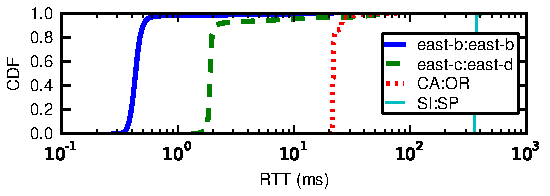
\includegraphics[width=\columnwidth]{graphs/ping-plot.pdf}
\caption{CDF of round-trip times for slowest inter- and intra-
  availability zone links compared to cross-region links.}
\label{fig:rtt}
\end{figure}


\subsection{CAP, Isolation, and Modern Systems}
\label{sec:modernacid}

Mitigating the effects of partitions and network latency is a
difficult task, requiring systems designers to make fundamental
trade-offs. In this section, we briefly discuss known semantic limits
for systems wishing to maintain high availability and their impact on
modern database systems. While the gold standard of ACID databases is
unavailable, we show that many database systems operate under much
weaker models, motivating the study of these models in a highly
available context in the remainder of this paper.

One of the most popularly celebrated impossibility results for
distributed systems is Brewer's CAP Theorem, which, as formally proven
by Gilbert and Lynch, states that it is impossible to maintain
linearizability (``C,'' or ``consistency''---albeit poorly named), or
the ability to read the last completed write, and replica availability
(``A'') in the presence of network partitions
(``P'')~\cite{gilbert-cap}. Brewer's Theorem has roots in decades of
distributed database designs~\cite{davidson-survey} and has had a
substantial impact on recent large-scale distributed systems design:
while CAP is narrowly scoped to the impossibility of building highly
available linearizable systems linearizability, it is often
interpreted to preclude a larger set of guarantees, including ACID, or
transactional atomicity, consistency, isolation and durability
guarantees, as evidenced by the lack of highly available systems
providing them.  As an example of an production database redesign
explicitly attributable to partition behavior, less than one year
after its announcement, Yahoo!'s PNUTS system developers explicitly
added a support for weaker, highly available operation, explaining
that ``strict adherence [to strong consistency] leads to difficult
situations under network partitioning or server failures...in many
circumstances, applications need a relaxed
approach''~\cite{pnuts-update}.

Database designers and researchers have long realized that
serializability---the gold standard of ACID isolation, which
guarantees application-level consistency---is not achievable in a
highly available system~\cite{davidson-survey}.  However, database
systems offer a range of ACID properties besides
serializability. Within a single-node database, the coordination
penalties associated with ensuring equivalence with a serial execution
can be severe and manifest themselves in the form of concurrency
control contention (and, subsequently, performance degradation,
scalability limitations, and, often, external aborts like
deadlocks)~\cite{gray-isolation}. Instead, databases offer a host of
so-called \textit{weak isolation} models that allow varying
restrictions on the space of schedules that are allowable by the
system~\cite{adya}. None of these weak isolation models guarantees
serializability, but the benefits of these models can often outweigh
costs of possible consistency anomalies that might arise
from their use.

To understand the prevalence of these weak isolation models, we
recently surveyed, we surveyed the default and maximum isolation
models provided by 18 relational databases, often claiming to provide
``ACID'' or ``NewSQL'' functionality~\cite{hat-hotos}. As shown in
Table~\ref{table:existing}, only three out of 18 databases provides
serializability by default, and at least eight do not provide
serializability as an option at all. This is particularly surprising
when we consider the widespread deployment of many of these
non-serializable databases, like Oracle 11g, which are known to power
major businesses and product functionality. Given that these
transactional models are frequently used, our inability to provide
serializability in arbitrary HATs is non-fatal for practical
applications. If application writers and database vendors have already
decided that the benefits of weak isolation outweigh potential
application inconsistencies, then, in a highly available environment
that prevents serializability entirely, similar decisions may be
appropriate.

\begin{table}
\begin{small}
\begin{tabular}{|l|c|c|}
\hline
Database & Default & Maximum\\\hline
Actian Ingres 10.0/10S & S & S\\
Aerospike & RC & RC\\
Akiban Persistit & SI & SI\\
Clustrix CLX 4100 & RR & ?\\
Greenplum 4.1 & RC & S \\
IBM DB2 10 for z/OS & CS & S\\
IBM Informix 11.50 & Depends & RR\\
MySQL 5.6 & RR & S \\
MemSQL 1b & RC & RC\\
MS SQL Server 2012 & RC & S \\
NuoDB & CR & CR\\
Oracle 11g & RC & SI\\
Oracle Berkeley DB & S & S\\
Oracle Berkeley DB JE & RR & S\\
Postgres 9.2.2 & RC & S\\
SAP HANA & RC & SI\\
ScaleDB 1.02 & RC & RC\\
VoltDB & S & S\\
\hline
\multicolumn{3}{|p{7cm}|}{{\footnotesize RC: read committed, RR: repeatable read, SI: snapshot isolation, S: serializability, CS: cursor stability, CR: consistent read}}\\\hline

\end{tabular}
\caption{Default and maximum isolation levels for ACID and NewSQL
  databases as of January 2013 (from
  \protect\cite{hat-hotos}).}\vspace{-1.5em}
\label{table:existing}
\end{small}
\end{table}

The primary challenge in providing weak isolation in a HAT context is
that, unfortunately, it is unclear \textit{which} of these isolation
guarantees can be provided with high availability. The existing
algorithms for providing weak isolation are typically designed for a
single-node context and are, to the best of our knowledge, unavailable
due to a reliance on concurrency control mechanisms like locking that
are not resilient to partial failure. Morever, we are not aware of any
prior literature that provides guidance as to the relationship between
weak isolation and high availability: prior work has examined the
relationship between serializability and high
availability~\cite{davidson-survey} and weak isolation on a
single-server~\cite{adya, ansicritique} but never weak isolation and
high availability taken together. We believe that this apparent gap in
the database literature is a possible contributing factor to the
often-apparent attitude that general-purpose transactional semantics
are either too expensive to provide in many modern distributed
databases---except under special circumstances, such as providing
operations over groups of co-located data items.



\section{High Availability}
\label{sec:availability}

To understand which guarantees can be provided with high availability,
we must first define what high availability means. In this section, we
will formulate a model that captures a range of availability models,
including high availability, availability with stickiness, and
transactional availability.

Informally, highly available algorithms ensure ``always on'' operation
and, as a side effect, guarantee low latency. If users of a highly
available system are able to contact a (set of) server(s) in a system,
they are guaranteed a response; this means servers will not need to
communicate with any others. If servers are partitioned from one
another, they do not need to stall in order to provide clients a
``safe'' response to operations. This lack of fast-path coordination
also means that a highly available system also provides low
latency~\cite{abadi-pacelc}; in a wide-area setting, clients of a
highly available system need not wait for cross-datacenter
communication. To properly describe whether a \textit{transactional}
system is highly available, we need to describe what servers a client
must contact as well as what kinds of responses a server can provide,
especially given the possibility of aborts.

\subsection{Replica Availability}

Traditionally, a system provides {\em high availability} if every user
that can contact a correct (non-failing) server eventually receives a
response from that server, even in the presence of arbitrary,
indefinitely long network partitions between
servers~\cite{gilbert-cap}.\footnote{Under this definition, systems
  that require a majority of servers to be online is not
  available. Similarly, a system which ensures that clients receive a
  response with high (but not perfect) probability is not
  available. This is a stringent definition but matches the
  assumptions made by the CAP Theorem~\cite{gilbert-cap} and
  guarantees low latency~\cite{abadi-pacelc}.} As in a standard
distributed database, designated servers might perform operations for
different data items; a server that can handle an operation for a
given data item is called a \textit{replica} for that
item.\footnote{There is a further distinction between a \textit{fully
    replicated} system, in which all servers are replicas for all data
  items, and a \textit{partially replicated} system, in which at least
  one server acts as a replica for only a subset of all data
  items. For generality, and, for applicability to many modern
  ``sharded'' or ``partitioned'' data storage systems~\cite{ bigtable,
    pnuts, spanner, dynamo, hstore}, we consider partially replicated
  systems.}

\subsection{Sticky Availability}

In addition to high availability, which allows operations on any
replica, distributed algorithms often assume a model in which clients
always contact the same logical (sets of) replica(s) across subsequent
operations. As we will discuss in Section~\ref{sec:hats}, clients can
ensure continuity between operations (e.g., reading their prior
updates to a data item) by maintaining affinity or ``stickiness'' with
a server or set of servers~\cite{vogels-defs}. In a fully-replicated
system, where all servers are replicas for all data items, stickiness
is simple: a client can maintain stickiness by contacting the same
server for each of its requests. However, in a partially-replicated
system, where servers are replicas for subsets of the set of data
items (which we consider in this paper), we say a client must remain
sticky with a single \textit{logical} server that may consist of
multiple physical servers.. We say that a system provides
\textit{sticky availability} if, whenever a client's operation on an
item is executed against a logical server that has observed all of its
prior operations, it eventually receives a response, even in the
presence of indefinitely long partitions. A client may choose to
become sticky available by acting as a server itself; for example, a
client might cache its reads and writes~\cite{bolton,
  sessionguarantees, swift}. Any guarantee achievable in a highly
available system is achievable in a sticky high availability system
but not vice-versa.

%% \begin{figure}
%% \centering
%% \begin{tikzpicture}[scale=0.8]
%%   \tikzstyle{every node}=[font=\small]
%%  \node[draw=none,fill=none] (1) at (0,0) {$1$-availability (high availability)}; 
%%  \node[draw=none,fill=none] (2) at (0,1) {$2$-availability}; 
%%  \node[draw=none,fill=none] (m-1) at (0, 2) {\ldots}; 
%%  \node[draw=none,fill=none] (m) at (0, 3) {majority availability}; 
%%  \node[draw=none,fill=none] (m+1) at (0, 4) {\ldots}; 
%%  \node[draw=none,fill=none] (n) at (0, 5) {$N$-availability}; 
%%  \node[draw=none,fill=none] (1s) at (4, 1.5) {$1$-sticky availability};
%%  \node[draw=none,fill=none] (2s) at (4, 2.5) {$2$-sticky availability};
%%  \node[draw=none,fill=none] (n2s) at (4, 3.5) {\ldots};
%%  \node[draw=none,fill=none] (n1s) at (4, 4.5) {$(N$$-$$1)$-sticky availability};

%%  \draw [->] (1) -- (2);
%%  \draw [->] (2) -- (m-1);
%%  \draw [->] (m-1) -- (m);
%%  \draw [->] (m) -- (m+1);
%%  \draw [->] (m+1) -- (n);
%%  \draw [->] (1) -- (1s);
%%  \draw [->] (1s) -- (m);
%%  \draw [->] (2s) -- (m+1);
%%  \draw [->] (1s) -- (2s);
%%  \draw [->] (2) -- (2s);
%%  \draw [->] (2s) -- (n2s);
%%  \draw [->] (n2s) -- (n1s);
%%  \draw [->] (n1s) -- (n);


%% \end{tikzpicture}
%% \caption{Hierarchy of replica availability levels for $N>3$ servers.}
%% \label{fig:availability-order}
%% \end{figure}

%% We show a hierarchy of replica availability levels in
%% Figure~\ref{fig:availability-order}. $K$-sticky availability subsumes
%% $K$-availability, but $K$-sticky availability is incomparable with
%% $(K+1)$-availability. $N$-sticky availability is equivalent to
%% $N$-availability, while majority availability subsumes $1$-sticky
%% availability. More generally, $\lceil \frac{N}{2} \rceil$$+$$K$$-$$1$
%% availability subsumes $K$-sticky availability. We have omitted
%% discussion of operation-specific availability levels (e.g.,
%% $N$-availability for writes and $1$-availability for reads in a
%% write-all, read-one data store), system membership changes, or
%% heterogeneous replicas (e.g., servers in a local and remote
%% datacenters) but believe there are several avenues for further
%% taxonomization.

\subsection{Transactional Availability}

Until now, we have considered single-object, single-operation
availability. This is standard in the distributed systems literature
(e.g., distributed register models such as linearizability all concern
single objects~\cite{herlihy-art}), yet the database literature
largely focuses on transactions: groups of multiple operations over
multiple objects. Accordingly, by itself, traditional definitions of
high availability are insufficient to describe availability guarantees
for transactions. Additionally, given the choice of \textit{commit}
and \textit{abort} responses---which signal transaction success or
failure to a client---we must take care in defining transactional
availability.

If a client wishes to execute a transaction that performs operations
on multiple data items, then the client must be able to contact and
receive a response from at least one replica for each data item. We
say that a transaction has \emph{replica availability} if it can
contact at least one replica for every item it attempts to
access. This may result in ``lower availability'' than a
non-transactional requirement. Additionally, given the possibility of
system-initiated aborts, we need to ensure useful forward progress: a
system can trivially guarantee clients a response by always aborting
all transactions. However, this is an unsatisfactory system because
nothing good (transaction commit) ever happens; we should require a
\textit{liveness} property~\cite{transaction-liveness}. We cannot
guarantee that every transaction will commit---transactions may choose
to abort themselves---but we need to make sure that the system will
not indefinitely abort transactions on its own volition. We call a
transaction abort due to a transaction's own choosing (e.g., as an
operation of the transaction itself or due to a would-be declared
integrity constraint violation) an \textit{internal abort} and an
abort due to system implementation or operation an \textit{external
  abort}. We say that a system provides \textit{transactional
  availability} if, given replica availability for every data item in
a transaction, the transaction eventually commits (possibly after
multiple client retries) or internally aborts~\cite{hat-hotos}.




\section{Highly Available Transactions}
\label{sec:hats}

HAT systems provide transactions with transactional availability and
either high availability or sticky high availability. They offer
substantial latency and availability benefits compared to traditional
distributed databases, yet they cannot achieve all the traditional
semantics. In this section, we delineate ACID, distributed
consistency, and session consistency levels which can be achieved with
high availability (transactional atomicity, variants of Repeatable
Read isolation, and many session guarantees), those with sticky high
availability (read your writes, PRAM and causal consistency) and the
properties which cannot be provided in a HAT system (those preventing
Lost Update and Write Skew, or with recency).  We present a full
summary of these results in Section~\ref{sec:hat-summary}.

As Brewer states, ``systems and database communities are separate but
overlapping (with distinct vocabulary)''~\cite{brewer-slides}. With
this challenge in mind, when possible, we build on existing properties
and definitions from the database and distributed systems literature,
providing a brief, informal explanation and example for each
guarantee. The database isolation guarantees require particular care,
since different DBMSs often use the same terminology for different
mechanisms and may provide additional guarantees in addition to our
implementation-agnostic definitions.  We draw largely on Atul Adya's
dissertation~\cite{adya} and somewhat on its predecessor work: the
ANSI SQL specification~\cite{ansi-sql} and Berenson et al.'s
subsequent 1995 critique~\cite{ansicritique}. We provide a set of
formal definitions, semantics, proofs and observations in our extended
Technical Report and opt for a more informal presentation in this
paper~\cite{hat-tr}.

\subsection{Achievable HAT Semantics}

To begin, we present well-known semantics that can be achieved in HAT
systems. We offer proof-of-concept highly available algorithms but our
goal is \textit{not} to provide optimal or even efficient
implementations. These guarantees are fairly straightforward and have
been introduced---albeit with greater brevity and discussion
omitted---in a preliminary workshop paper~\cite{hat-hotos}. In our
examples, we exclusively consider read and write operations. We denote
a write of value $v$ to data item $d$ as $w_d(v)$ and a read from data
item $d$ returning $v$ as $r_d(v)$ and assume that all data items have
the null value, $\bot$, at database initialization. Unless otherwise
specified, all example transactions commit.

\subsubsection{ACID Isolation Guarantees}

To begin, \textbf{Read Uncommitted} isolation is captured by Adya as
PL-1,requiring that each transaction's writes are ordered consistently
according to a single total order on transactions. This prohibits
Adya's phenomenon $G0$, also called ``Dirty Writes''~\cite{adya}. If
two transactions write to the same set of data items, then the final
database state cannot contain the ``earlier'' transaction's writes to
the data items. For example, in the below example, $T_3$ should
\emph{eventually} only read $a=b=1$ or $a=b=2$ but not $a=2, b=1$ or
$a=1, b=2$:
\begin{align*}
\small
T_1 &: w_x(1)~w_y(1)
\\T_2 &: w_x(2)~w_y(2)
\\T_3 &: r_x(a)~r_y(b)\\[-2em]
\end{align*}
All later properties will strengthen PL-1.

Unlike the total order required by serializability, the order in PL-1
does not constrain the values seen in by a transaction's read
operations except once the database has reached a ``final
state.'' Read Uncommitted is easily achieved via applying the same
logical timestamp to each update in a transaction and applying a
``last writer wins'' conflict reconciliation policy at each replica.

\textbf{Read Committed} isolation is particularly important in
practice as it is the default of many DBMSs. Implementations differ,
with some based on long-duration exclusive locks and short-duration
read locks~\cite{gray-isolation} and others based on multiple
versions. The implementations typically have recency and monotonicity
properties beyond the simple meaning of the name, which is what is
expressed in the implementation-agnostic definition: under Read
Committed, transactions should do not access uncommitted or
intermediate versions of data items. This prohibits both ``Dirty
Writes'', as above, and also ``Dirty Reads'' phenomena.  This
isolation is Adya's PL-2, and formalised by prohibiting Adya's $G1a-c$
(or ANSI's $P1$, or ``broad'' $P1$ (2.2) from Berenson et al.). For
instance, in the example below, $T_3$ should never see $a=1$, and, if
$T_2$ aborts, $T_3$ should never read $a=3$:
\vspace{-.5em}
\begin{align*}
\small
T_1 &: w_x(1)~w_x(2)
\\T_2 &: w_x(3)\\
T_3 &: r_x(a)\\[-2em]
\end{align*}
It is fairly easy for a HAT system to prevent ``Dirty Reads'': if each
transaction never writes uncommitted data to the database, then
transactions will never read each others' dirty data. As a simple
solution, clients can buffer their writes until they commit, or,
alternatively, can send them to servers, who will not deliver their
value to other readers until notified that the writes have been
committed. This implementation does not provide recency or
monotonicity guarantees but satisfies the implementation-agnostic
definition.

``Repeatable Read'' isolation is a confusing property. Some IBM
products use the term for fully serializable
isolation~\cite{hat-hotos}. Gray~\cite{gray-isolation}, Berenson et
al.~\cite{ansicritique}, and Adya's PL-2.99~\cite{adya} all interpret
Repeatable Read as providing serializability for all operations except
predicate-based reads (and so Repeatable Read is identical to
serializability in a key-value store without predicate-based
access). In this model, the \textit{Phantom Problem}, whereby two
successive predicate-based reads return different
data~\cite{gray-isolation}, is the only kind of non-serializable
behavior allowed. When referring to ``Repeatable Read,'' we will
follow these definitions, which, as we will soon show, are for a
property that can be offered in a highly available way.

However, As Berenson et al.~\cite{ansicritique} discuss, the ANSI SQL
specification allows many additional behaviors under the term
Repeatable Read isolation.  \textbf{ANSI Repeatable Read} requires
that, along with respecting Read Committed isolation, each transaction
will only read one version of each data item that it did not itself
produce (preventing ``Fuzzy Read,'' or P2). In the example below,
$T_3$ must read $a=1$:
\begin{align*}
\small
T_1 &: w_x(1)
\\T_2 &: w_x(2)
\\T_3 &: r_x(1)~r_x(a)
\end{align*}
This is a literal interpretation of the phrase ``Repeatable Read'':
unless a transaction modifies a given data item, the observable value
of the data item should not change during the transaction. By itself,
this property is extremely weak---we can always read $\bot$ for each
data item---and easily achieved in a HAT system by caching the values
read.

Between our Repeatable Read (PL-2.99) and the ANSI definition, is a
concept we will call \textbf{Item Cut Isolation}: that all the
transaction's reads should see values from a non-changing consistent
cut or snapshot over the data items. It is possible to satisfy Item
Cut Isolation with high availability by using multi-versioning on each
replica and ensuring that each of a transaction's reads return an
appropriately chosen version (e.g., identified by vector clock).

A stronger achievable property asks that a consistent cut spans both a
transaction's predicate reads (e.g., \texttt{SELECT WHERE}) as well as
its item reads.  We call this \textit{Predicate Cut
  Isolation}\footnote{Oracle provides an isolation level called
  ``Statement Level Read Consistency''~\cite{adya}; this is analogous
  to Predicate Cut Isolation at the level of a single operation within
  a multi-operation transaction. We do not consider this isolation
  model here as it is subsumed by standard Snapshot Isolation and we
  believe our discussion is easily extended to incorporate it.} and it
prohibits Phantoms. Predicate Cut Isolation is also achievable in HAT
systems via similar multi-versioning as above.

\subsubsection{ACID Atomicity Guarantees}

Transactional atomicity (TA) is core to ACID guarantees. Although, at
least by the ACID acronym, it is not an ``isolation'' property,
transactional atomicity restricts the ability to view the effects of
partially completed transactions. Under transactional atomicity, once
some of the effects of a transaction $T_1$ are observed by another
transaction $T_2$, thereafter all effects of $T_1$ are observed by
$T_2$. Together with item cut isolation, TA prevents Read Skew
anomalies (Berenson et al.'s A5A~\cite{ansicritique}). As an example
of TA, because $T_2$ has read $T_1$'s write to $y$, $T_2$ must observe
$b=c=1$ (or later versions for each key):
\vspace{-.5em}
\begin{align*}
\small
T_1 &: w_x(1)~w_y(1)~w_z(1)
\\T_2 &: r_x(a)~r_y(1)~r_x(b)~r_z(c)~\\[-1.5em]
\end{align*}
$T_2$ can also observe $a=\bot$, $a=1$, or a later version of
$a$. Notably, TA requires Read Committed isolation: observing all
effects of a transaction implicitly requires observing the final
(committed) effects of a transaction as well.

Perplexingly, discussions of TA are absent from existing ones of
weak isolation. This is perhaps again due to the single-node
context in which prior work was developed: on a single server (or a
fully replicated database), TA is achievable via lightweight locking
and/or local concurrency control over data items~\cite{gstore}. In
contrast, in a distributed environment, TA over arbitrary groups of
non-colocated items is considerably more difficult to achieve with
high availability: servers need to know when all of a transaction's
updates are present on their respective replicas. However, replicas do
not need to agree on when to reveal a new value to clients, which
would require consensus; accordingly, TA only requires reliable
broadcast (with some additional client metadata) and is
achievable in HAT systems. We omit a full discussion of the algorithm
and instead refer the reader to the extended version of this
paper~\cite{hat-tr}.  
%space{.5em}

\subsubsection{Session Guarantees}

Our models have not yet considered interactions \textit{across}
transactions: we have not guaranteed any ordering or continuity
between transactions, other than that there exists some arbitrary
ordering (via Read Uncommitted). In the distributed systems
literature, many useful \textit{safety} guarantees span multiple
application actions. In particular, \textit{session guarantees} are
used to describe guarantees across transactions within a given
\textit{session}, ``an abstraction for the sequence of...operations
performed during the execution of an
application''~\cite{sessionguarantees}. Informally a session describes
a context that should persist between transactions: for example, on a
social networking site, all of a user's transactions submitted between
``log in'' and ``log out'' operations might form a session.

There are several session guarantees that we can make with high
availability:

\vspace{.5em}\noindent\textit{{Monotonic reads}} requires that, within
a session, subsequent reads to a given object ``never return any
previous values''; reads from each item progress forward in a total
order. The ordering of reads should respect any externally observable
total ordering on transactions.

\vspace{.5em}\noindent\textit{{Monotonic writes}} requires that each
session's writes be applied to any replica in the order they were
submitted by the client. Any order on transactions should also be
consistent with any precedence that a global observer would see.

\vspace{.5em}\noindent\textit{{Writes Follow Reads}} requires that, if
a session observes an effect of transaction $T_1$ and subsequently
commits transaction $T_2$, then another session can only observe
effects of $T_2$ if it can also observe $T_1$'s effects (or later
values that supercede $T_1$'s).  Any order on transactions should
respect the reads-from order.\vspace{.5em}

The above guarantees can be achieved by forcing servers to wait to
reveal new writes until each write's respective dependencies are
fulfilled on all replicas. This mechanism effectively ensures that all
clients read from a globally agreed upon lower bound on the versions
written. This \textit{is} highly available as a client
will never block due to inability to find a server with a sufficiently
up-to-date version of a data item. However, it does not imply that
transactions will read their own writes or, in the presence of
partitions, make forward progress through the version history. The
problem is that, if a server becomes partitioned, under the highly
available model, we must handle the possibility that an unfortunate
client will be forced to issue her next requests against the
partitioned server.

The solution to this conundrum is to give up high availability in
favor of sticky availability. Sticky availability permits three
additional models, which we first define and then prove are
unachievable in a generic highly available system:

\vspace{.5em}\noindent\textit{{Read your writes}} requires
that whenever a client reads a given data item after updating it, the
read returns the updated value (or a value with a higher ID).

\vspace{.5em}\noindent\textit{{PRAM}} (Pipelined Random Access
Memory) provides the illusion of serializing each session's operations
and is the combination of monotonic reads, monotonic writes, and read
your writes~\cite{herlihy-art}.

\vspace{.5em}\noindent\textit{{Causal
    consistency}}~\cite{causalmemory} is the combination of all of the
session guarantees~\cite{sessiontocausal} (alternatively, PRAM with
writes-follow-reads) and is also referred to by Adya as PL-2L
isolation~\cite{adya}).\vspace{.5em}


Read your writes is not achievable in a highly available
system. Consider a client that executes the following two transactions
in succession:
\vspace{-.5em}
\begin{align*}
\small
T_1 &: w_x(1)
\\T_2 &: r_x(a)
\end{align*}
If the client executes $T_1$ against a server that is partitioned from
the rest of the other servers, the server must allow $T_1$ to
commit. If the client executes $T_2$ against the same (partitioned)
server, then it will be able to read its writes. However, if the
network topology shifts and the client can only contact a different
server that is partitioned from the server that executed $T_1$, then
the client will be unable to read its own writes and the system will
have to either stall indefinitely to allow the client to read her
writes (violating transactional availability) or will have to
sacrifice read your writes guarantees. However, if the client remains
sticky with the server that executed $T_1$, then we can disallow this
scenario. Accordingly, read your writes, and, by proxy, causal
consistency and PRAM require stickiness. Read your writes is ``free''
in a sticky system, while the remaining causality and PRAM guarantees
can be accomplished with the algorithms for achieving the remaining
session guarantees.

\subsubsection{Additional HAT Guarantees}

In this section, we briefly discuss additional noteworthy guarantees
achievable by HAT systems.

\noindent{\textbf{Consistency}} A HAT system can make limited
consistency guarantees. It can often execute commutative and logically
monotonic~\cite{calm} operations without the risk of invalidating
(also monotonic) application-level integrity constraints. Our goal in
this paper is not to sketch the entire space of consistency models
that are achievable (see Section~\ref{sec:futurework}). We
specifically evaluate TPC-C transaction semantics under HAT
consistency guarantees in Section~\ref{sec:evaluation}.

\vspace{.5em}\noindent{\textbf{Durability}} A client requiring that its
transactions' effects survive $F$ server faults requires at least
$F+1$ correct nodes.

\vspace{.5em}\noindent{\textbf{Convergence}} To require that the
system propagates writes between replicas, we can require convergence,
or eventual consistency for each data item: in the absence of new
mutations to a data item, in the absence of partitions, all servers
should eventually agree on the value for each item. This is typically
accomplished by any number of anti-entropy protocols, which
periodically update neighboring servers with the latest value for each
data item~\cite{antientropy}. Establishing a final value is related to
determining a total order on transaction updates, as in Read
Uncommitted.

\subsection{Unachievable HAT Semantics}
\label{sec:unachievable-hat}

While there are infinitely many HAT models
(Section~\ref{sec:futurework}), at this point, we have largely
exhausted the range of achievable, previously defined (and useful)
semantics that are available to HAT systems. Before summarizing our
possibility results, we will present impossibility results for HATs,
also defined in terms of previously identified isolation and
consistency anomalies. Most notably, it is impossible to
prevent Lost Update or Write Skew in a HAT system.

\subsubsection{Unachievable ACID Isolation}

In this section, we demonstrate that preventing Lost Update and Write
Skew---and therefore providing Snapshot Isolation, Repeatable Read,
and one-copy serializability---inherently requires unavailability.

In the words of Berenson et al., \textit{Lost Update} occurs when one
transaction $T1$ reads a given data item, a second transaction $T2$
updates the same data item, then $T1$ modifies the data item based on
its original read of the data item, ``missing'' or ``losing'' $T2$'s
newer update. Consider a database containing only the following
transactions:
\begin{align*}
\small
T_1 &: r_x(a) w_x(a+2)
\\T_2 &: w_x(2)
\end{align*}
If $T_1$ reads $a=1$ but $T_2$'s write to $x$ precedes $T_1$'s write
operation, then the database will end up with $a=3$, a state that
could not have resulted in a serial execution due to from $T_2$'s
``Lost Update.''

It is impossible to prevent Lost Update in a highly available
environment. Consider two clients who submit the following $T_1$ and
$T_2$ on opposite sides of a network partition:
\begin{align*}
\small
T_1 &: r_x(100)~w_x(100+20=120)
\\T_2 &: r_x(100)~w_x(100+30=130)
\end{align*}
Regardless of whether $x=120$ or $x=130$ is chosen by a replica, the
database state could not have arisen serial execution of $T_1$ and
$T_2$.\footnote{In this example, we assume that, as is standard in
  modern databases, replicas accept values as they are written (i.e.,
  register semantics). This particular example could be made
  serializable via the use of commutative updates
  (Section~\ref{sec:eval}) but, as we show in the extended version of
  the paper~\cite{hat-tr}, the problem persists in the general case.}
To prevent this from happening, either $T_1$ or $T_2$ should not have
committed. Each client's respective server might try to detect that
another write occurred, but this requires knowing the version of the
latest write to $x$. In our example, this reduces to a requirement for
linearizability, which is, via Gilbert and Lynch's proof of the CAP
Theorem, provably unachievable with high
availabilty~\cite{gilbert-cap}.

\textbf{Write Skew} is a generalization of Lost Update to multiple
keys. It occurs when one transaction $T1$ reads a given data item $x$,
a second transaction $T2$ reads a different data item $y$, then $T1$
writes to $y$ and commits and $T2$ writes to $x$ and commits. As an
example of Write Skew, consider the following two transactions:
\begin{align*}
\small
T_1 &: r_y(0)~w_x(1)
\\T_2 &: r_x(0)~w_y(1)
\end{align*}
As Berenson et al. describe, if there was an integrity constraint
between $x$ and $y$ such that only one of $x$ or $y$ should have value
$1$ at any given time, then this write skew would violate the constraint (which is preserved in serializable executions). Write skew is a somewhat
esoteric anomaly---for example, it does not appear in
TPC-C~\cite{snapshot-serializable}---but, as a generalization of Lost
Update, it is also unavailable to HATs.

Their need to prevent Lost Update means that Consistent Read, Snapshot
Isolation, and Cursor Stability guarantees are all unavailable.
Repeatable Read (in the sense of Gray~\cite{gray-isolation}, Berenson
et al.~\cite{ansicritique}, or Adya~\cite{adya}) and One-Copy
Serializability need to prevent both Lost Update and Write Skew; this
means that they are also inherently unavailable.

\subsubsection{Unavailable Recency Guarantees}

Data storage systems make various recency guarantees on reads of data
items. As we have discussed, one of the most famous is
linearizability~\cite{herlihy-art}, which states that reads will
return the last completed write to a data item, and there are several
other (weaker) variants such as safe and regular register
semantics. When applied to transactional semantics, the combination of
one-copy serializability and linearizability is called \textit{strong
  (or strict) one-copy serializability}~\cite{adya} (e.g., Google's
Spanner~\cite{spanner}). It is also common, particularly in systems
that allow reading from masters and slaves, to provide a guarantee
such as ``read a version that is no more than five seconds out of
date'' or similar. Unfortunately, an indefinitely long partition can
force an available system to violate any recency bound, so recency
bounds are not enforceable in HAT systems.

\subsection{Summary}
\label{sec:hat-summary}

We summarize our results in Table~\ref{table:hatcompared}. A wide
range of isolation levels are achievable in a HAT systems, including
transactional atomicity, cut isolation, and several session
guarantees. With sticky availability, a system can achieve read your
writes guarantees and PRAM and causal consistency. However, many other
prominent models, such as Snapshot Isolation, One-Copy
Serializability, and Strict Serializability cannot be achieved due to
the inability to prevent Lost Update and Write Skew phenomena.

We illustrate the hierarchy of available, sticky available, and
unavailable consistency models we have discussed in
Figure~\ref{fig:hatcompared}. Many models are simultaneously
achievable, but we find several particularly compelling. If we combine
all sticky-HAT guarantees, we have transactional, causal snapshot
reads (i.e., Causal Transactional Predicate Cut Isolation). If we
combine TA and P-CI, we have transactional snapshot reads. We can
achieve RC, MR, and RYW by simply sticking clients to servers. And we
can also combine unavailable models---for example, an unavailable
system might provide PRAM and One-Copy
Serializability~\cite{daudjee-session}.

To the best of our knowledge, this is the first unification of
database ACID, distributed consistency, and session guarantee
models. Interestingly, strong one-copy serializability subsumes all
other models, while considering the (large) power set of all
compatible models (e.g., the diagram depicts 96 possible highly
available combinations) hints at the vast expanse of consistency
models found in the literature. This taxonomy  is \textit{not}
exhaustive, but we believe it lends substantial clarity into the
relationships between a large subset of the prominent ACID and
distributed consistency models. Additional read/write transaction
semantics that we have omitted should be easily classifiable based on
the available primitives and HAT-incompatible anomaly prevention we
have already discussed.

 \newcommand{\lostupdate}{$^\dagger$}
 \newcommand{\rwskew}{$^\ddagger$}
 \newcommand{\linearizable}{$^\oplus$}

\begin{table}[t!]
\begin{tabular}{| c | p{6cm} | }\hline
HA & Transactional Atomicity (TA), Read Uncommitted (RU), Read
Committed (RC), Item Cut Isolation (P-CI), Predicate Cut Isolation
(P-CI), Monotonic Reads (MR), Monotonic Writes (MW), Writes Follow
Reads (WFR)\\\hline Sticky-HA & Read Your Writes (RYW), PRAM,
Causal\\\hline Unavailable & Cursor Stability (CS)\lostupdate,
Snapshot Isolation (SI)\lostupdate, Repeatable Read
(RR)\lostupdate\rwskew, One-Copy Serializability
(1SR)\lostupdate\rwskew, Recency\linearizable, Safe\linearizable,
Regular\linearizable, Linearizability\linearizable, Strong
1SR\lostupdate\rwskew\linearizable \\\hline
\end{tabular}
\caption{Summary of highly available, sticky highly available, and
  unavailable models considered in this paper. Unavailable models are
  labeled by cause of unavailability: preventing lost
  update\lostupdate, preventing write skew\rwskew, and requiring
  recency guarantees\linearizable.}
\label{table:hatcompared}
\end{table}

\begin{figure}[t!]
\centering
\begin{tikzpicture}[scale=0.8]
  \tikzstyle{sticky}=[rectangle,draw=blue!50,fill=blue!20,thick]
  \tikzstyle{noha}=[ellipse,draw=red!50,fill=red!20,thick, inner sep=0pt,minimum size=12pt]

  \tikzstyle{every node}=[font=\small]

 \node[draw=none,fill=none] (ici) at (1.2, 0) {I-CI};
 \node[draw=none,fill=none] (pci) at (1.65, 1.2) {P-CI};
 \node[draw=none,fill=none] (rc) at (-1.2, .8) {RC};
 \node[draw=none,fill=none] (ru) at (-1.2, 0) {RU};

 \node[draw=none,fill=none] (ta) at (-.2, 1.3) {TA};

 \node[draw=none,fill=none] (mr) at (3.6, 0) {MR};
 \node[draw=none,fill=none] (mw) at (4.8, 0) {MW};
 \node[draw=none,fill=none] (wfr) at (2.4,0) {WFR};
 \node at (6.1,0) [sticky] (ryw) {RYW};

 \node[noha](recency) at (7.7, 0) {recency};
 \node[noha](safe) at (7.7, 1) {safe};
 \node[noha](regular) at (7.7, 2) {regular};
 \node[noha](linearizable) at (7.7, 3) {linearizable};
 \node at (4.8, 2) [sticky] (causal) {causal};
 \node at (4.8, 1) [sticky] (pram) {PRAM};
 \node[noha] (cs) at (-1.2, 1.8) {CS};
 \node[noha] (rr) at (-.2, 2.7) {RR};
 \node[noha] (si) at (2.2, 2.4) {SI};
 \node[noha] (1sr) at (1.2, 3.2) {1SR};
 \node[noha] (ssr) at (3.85, 3.6) {Strong-1SR};

 \draw [->, red] (recency) -- (safe);
 \draw [->, red] (safe) -- (regular);
 \draw [->, red] (regular) -- (linearizable);
 \draw [->, red] (linearizable) -- (ssr);
 \draw [->, red] (1sr) -- (ssr);
 
 \draw [->] (ru) -- (rc);
 \draw [->] (rc) -- (ta);
 \draw [->] (ici) -- (pci);

 \draw [->, blue] (mr) -- (pram);
 \draw [->, blue] (mw) -- (pram);
 \draw [->, blue] (wfr) -- (causal);
 \draw [->, blue] (ryw) -- (pram);
 \draw [->, blue] (pram) -- (causal);

 %\draw[snake=coil, segment aspect=0, segment amplitude=.75pt, segment length=2pt] (ru) -- (mr);
 %\draw[snake=coil, segment aspect=0, segment amplitude=.75pt, segment length=2pt] (rc) -- (ta);
 %\draw[snake=coil, segment aspect=0, segment amplitude=.75pt, segment length=2pt] (ici) -- (ta);
 %\draw[snake=coil, segment aspect=0, segment amplitude=.75pt, segment length=2pt] (pci) -- (ta);
 %\draw[snake=coil, segment aspect=0, segment amplitude=.75pt, segment length=2pt] (rc) -- (mr);
 %\draw[snake=coil, segment aspect=0, segment amplitude=.75pt, segment length=2pt] (pci) -- (mr);
 %\draw[snake=coil, segment aspect=0, segment amplitude=.75pt, segment length=2pt] (ici) -- (mr);
 %\draw[snake=coil, segment aspect=0, segment amplitude=.75pt, segment length=2pt] (ta) -- (ru);
 %\draw[snake=coil, blue, segment aspect=0, segment amplitude=.75pt, segment length=2pt] (ru) -- (causal);
 %\draw[snake=coil, segment aspect=0, segment amplitude=.75pt, segment length=2pt] (mr) -- (mw);
 %\draw[snake=coil, segment aspect=0, segment amplitude=.75pt, segment length=2pt] (wfr) -- (mw);
 %\draw[snake=coil, blue, segment aspect=0, segment amplitude=.75pt, segment length=2pt] (wfr) -- (ryw);

 \draw [->, red] (rc) -- (cs);
 \draw [->, red] (cs) -- (rr);
 \draw [->, red] (pci) -- (si);
 \draw [->, red] (ici) -- (rr);
 \draw [->, red] (rr) -- (1sr);
 \draw [->, red] (si) -- (1sr);
 \draw [->, red] (ta) -- (si);
 \draw [->, red] (ta) -- (rr);
 \draw [->, red] (causal) -- (linearizable);
 \draw [->, red] (ryw) -- (safe);

\end{tikzpicture}
\label{fig:hat-order}
\caption{HAT, sticky HAT (in boxes), and unavailable models (circled)
  from Table~\protect\ref{table:hatcompared} compared
  graphically. Directed edges represent ordering by model
  strength. Models that do not share a common ancestor can be
  simultaneously achieved, and the resulting availability is that of
  the weakest available model in the combination.}
\label{fig:hatcompared}
\end{figure}


\subsection{Discussion}
\label{sec:discussion}

In this section, we discuss several subtleties in our results,
specifically addressing model composition, transactional atomicity
versus linearizability, and stickiness requirements.

\vspace{.5em}\noindent\textbf{Model Composition} Choosing between
combinations of compatible guarantees requires care. Consider the
following transactions:
\begin{align*}
\small
T_1 &: w_x(1)~w_y(1)
\\T_2 &: w_x(2)~w_y(2)
\\T_3 &: r_x(a)~r_y(b)
\end{align*}
If we want to guarantee both cut isolation and transactional atomicity
and the system only executes $T_1$, $T_2$, and $T_3$, then $T_3$ needs
to read $a=b=\bot$, $a=b=1$, or $a=b=2$. This means that either the
implementation should frequently return $\bot$ (definitely undesirable
and possibly non-convergent), keep multiple versions of each data item
(necessitating potentially complicated distributed garbage
collection), or use pre-declared read sets to fetch a consistent cut
of keys before each transaction begins to execute. Using client-side
caching can alleviate some of these challenges~\cite{bolton, swift},
but then the system becomes sticky high available.

Composition cost also varies by combination. For instance, Charron-Bost
has proven that, to capture causality between $N$ communicating
processes, standard vector-based approaches face an upper bound of
$O(N)$ storage per write~\cite{charron-bost}. This means that, with
$100K$ clients, each write might be accompanied by $100K$ timestamps
per vector. This is difficult to scale. By compromising on
availability (e.g., treating a datacenter as a linearizable cluster),
this overhead can be reduced~\cite{eiger}, but it is much
cheaper to provide, say, read your writes, than full causal
consistency.

\vspace{.5em}\noindent\textbf{Linearizability and Transactional
  Atomicity} The relationship between linearizability and
transactional atomicity is non-obvious. Transactional atomicity
dictates that writes to multiple keys across multiple servers are made
visible to readers all at once, while linearizability dictates that
writes to a single key on multiple servers are made visible to all
readers at once---what is different? First, in linearizable (and safe
and regular) systems, writes are made visible to all clients
\textit{immediately} after they finish. With transactional atomicity,
there is no recency guarantee. Second, in linearizabile systems, all
clients see all writes at the same time. With transactional atomicity,
clients may see writes at different times depending on which replicas
they contact. We are not aware of an analogous model in the
distributed systems literature. Accordingly, despite apparent
similarities, transactional atomicity is incomparable with and much
cheaper (by availability standards) than linearizability.

\vspace{.5em}\noindent\textbf{Visibility and Stickiness} Sticky
availability can result in much better write \textit{visibility}:
clients will be able to safely read writes more quickly in a sticky
available system. In the model we discussed, it is possible to achieve
several properties like monotonic reads in a highly available system
by waiting to reveal a write until all servers have seen it and its
relevant dependencies. However, this incurs severe visibility
penalties---new writes will not become visible to clients in the
presence of partitions. A client that does not want to guarantee
read-your-writes (due to the sticky availability requirement) may
still wish to read other clients' writes with timeliness.



\section{HAT Implications}
\label{sec:evaluation}

With an understanding of which guarantees are HAT-compliant, in this
section, we analyze the implications of these results for existing
systems and briefly study HAT systems on public cloud
infrastructure. Specifically:

\begin{myenumerate}
\item We revisit traditional database concurrency control with a focus
  on coordination costs and on high availability.
\item We examine the properties required by a realistic OLTP
  application based on the TPC-C benchmark.
\item We perform a brief experimental evaluation of HAT versus non-HAT
  properties on public cloud infrastructure.
\end{myenumerate}

\subsection{Existing Algorithms}

Many existing database transaction and concurrency control algorithms
are not designed for high availability. These algorithms often presume
a single-server deployment or a requirement for serializability. As
a consequence, traditional transaction processing systems are not
well-optimized for a HAT context. In this section, we briefly discuss
design decisions and algorithmic details that preclude high
availability.

\vspace{.5em}\noindent\textbf{Serializability} To establish a serial
order on transactions, algorithms for achieving serializability of
general-purpose read-write transactions in a distributed
setting~\cite{bernstein-book} may require at least one round trip time
(RTT) before committing. As an example, traditional two-phase locking
for a transaction of length $T$ may require $T$ \texttt{lock}
operations and will require at least one \texttt{lock} and
\texttt{unlock} operation.  In a distributed environment, each of
these operations requires coordination, either with other database
replicas or with a lock service. If this coordination mechanism is
unavailable, transactions cannot safely commit. Similarly, optimistic
concurrency control requires coordinating via a validation step, while
deterministic transaction scheduling~\cite{deterministic-scheduling}
requires a scheduler. Serializability under multi-version concurrency
control also requires checking for update conflicts. The reliance on a
globally agreed total order necessitates a minimum of one round-trip
to a designated master or coordination service for each of these
classic algorithms.  The cost of the (minimum one) round trip will be
determined by the deployment environment, as we saw in
Section~\ref{sec:motivation}; we will demonstrate this cost on public
cloud infrastructure in the next section.

\vspace{.5em}\noindent\textbf{Non-serializability} Many existing
distributed implementations of weak isolation are not highly
available. Lock-based proposals such as those used to provide weak
isolation in Gray's original proposal~\cite{gray-isolation} do not
degrade gracefully in the presence of partial failures. (Note, however,
that lock-based protocols \textit{do} offer the benefit of recency
guarantees.) While multi-versioned storage systems allow for a variety
of transactional guarantees, we have not seen proposals for truly weak
isolation (e.g., non-``tentative update'' schemes) in this context.
The MDCC~\cite{mdcc} protocol offers Read Committed isolation with
Lost Update avoidance but is similarly unavailable due to its reliance
on preventing write conflicts. Chan and Gray's read-only transactions
provide read-only transactions with item-cut isolation, causal
consistency, and transactional atomicity (session PL-2L~\cite{adya})
but are unavailable in the presence of coordinator
failure~\cite{readonly}, similar to read-only and write-only
transactions more recently proposed by Eiger~\cite{eiger}; Causal
Serializability offers a similar model (with unavailable
implementation): causal consistency with a variant of Read Uncommitted
between transactions that write to the same data
item~\cite{raynal-causal}.  Bolt-on causal consistency~\cite{bolton},
Brantner's S3 database~\cite{kraska-s3}, and
Bayou~\cite{sessionguarantees} can all provide variants of session
PL-2L with high availability, but none provide this HAT functionality
without substantial modification; Swift~\cite{swift} is closest to
providing full HAT operation in a sticky context. As  seen, it
is possible to implement many guarantees weaker than
serializability---including guarantees that are achievable with high
availability---and still not achieve high availability.

\subsection{Application Requirements}

Thus far, we have largely ignored the question of which applications
require semantics that are unavailable to HATs. As we showed in
Section~\ref{sec:hats}, the main cost of choosing HATs comes in the
inability to prevent Lost Update, Write Skew, and provide recency
bounds. In this section, we attempt to understand when these
guarantees matter both abstractly and in a representative
transactional application based on the TPC-C benchmark~\cite{tpcc}.

\vspace{.5em}\noindent\textbf{Commutativity and Monotonicity} Recent
work on the CALM Theorem~\cite{calm} and Commutative and Replicated Data
Types~\cite{crdt} demonstrates that, if updates logically commute,
then they can often be safely performed in different orders at
different replicas. Accordingly, as long as all writes are delivered
to all replicas, then a system executing monotonic logic with
commutative operators may not suffer from application-level
consistency anomalies as a result of Lost Update or Write Skew
anomalies. However, applications with non-monotonic state mutation
will not, in general, be able to maintain application-level
consistency constraints with HATs alone. Moreover, applications with
requiring bounded update visibility latency should opt for
unavailability.

\vspace{.5em}\noindent\textbf{TPC-C} To better understand the impact
of HAT-compliance in an application context, we consider a concrete
application: the TPC-C benchmark. Surprisingly, four of five
transactions can be executed with HATs, while the fifth may require
unavailablity.

TPC-C consists of five transactions, capturing the operation of a
wholesale warehouse, including sales, payments, and deliveries. Two
transactions---\textit{Order-Status} and \textit{Stock-Level}---are
read-only and can be executed safely under HATs. Clients may read
stale data, but this does not violate TPC-C requirements and clients
will read their writes if they are sticky-available. Another
transaction type, \textit{Payment}, updates running balances for
warehouses, districts, and customer records as well as providing an
audit trail. The transaction is increment- and append-only, so all
balance increase operations commute, and TA allows the
maintainence of any foreign-key constraints (e.g.,
\texttt{UPDATE/DELETE CASCADE}).

While three out of five transactions are easily achievable with
HATs, the remaining two transactions---\textit{New-Order} and
\textit{Delivery}---are not as simple. The New-Order transaction
places an order for a variable quantity of data items, updating
warehouse stock as needed. It selects a sales district, assigns the
order an ID number, adjusts the remaining warehouse stock, and writes
a placeholder entry for the pending order. The Delivery transaction
represents the fulfillment of a New-Order: it deletes the order from
the pending list, updates the customer's balance, updates the order's
carrier ID and delivery time, and updates the customer balance.

New-Order presents two challenges: ID assignment and stock
maintainence. First, each New-Order transaction requires a unique ID
number for the order. We can create a unique number by, say,
concatenating the client ID and a timestamp. However, the TPC-C
specification requires order numbers to be \textit{sequentially}
assigned within a district, which requires preventing Lost
Update. Accordingly, HATs cannot provide compliant TPC-C execution but
can maintain uniqueness constraints. Second, the New-Order transaction
decrements inventory counts: what if the count becomes negative?
Fortunately, TPC-C New-Order restocks each item's inventory count
(increments by 91) if it would become negative as the result of
placing an order. This means that, even in the presence of concurrent
New-Orders, an item's stock will never fall below zero. This is TPC-C
compliant, but a HAT system might end up with much more stock
than in a non-HAT-compliant implementation.

Delivery is challenging due to non-monotonicity. Each Delivery deletes
a pending order from the NewOrder Table and should be idempotent in
order to avoid billing a customer twice; this implies a need to
prevent Lost Update. This issue  can be avoided  by moving the
non-monotonicity to the real world---the carrier that picks up the
package for an order can ensure that she is the only carrier who has
done so---but cannot provide a correct execution with HATs
alone. However, according to distributed transaction
architects~\cite{entitygroup}, these compensatory actions are
relatively common in real-world business processes.

Throughout execution, TPC-C also requires the maintainence of several
integrity constraints. For example, Consistency Condition 1 (3.3.2.1)
requires that each warehouse's sales count must reflect the sum of its
subordinate sales districts. This integrity constraint spans two
tables but, given the ability to update rows in both tables atomically
via transactional atomicity, can be easily maintained. Consistency
Conditions 4 through 12 (3.3.2.4-12) can similarly be satisfied by
applying updates atomically across tables. Consistency Conditions 2
and 3 (3.3.2.2-3) concern order ID assignment and are more
problematic, as we have discussed.  Finally, while TPC-C is not
subject to multi-key anomalies, we note that many TPC-E isolation
tests, such as one that requires simultaneously modifying a product
description and its image, are also passable using HATs.

In summary, many---but not all---TPC-C transactions are well-served by
HATs. The two problematic transactions---New-Order and Payment---rely
on non-monotonic state update. The former transaction can be modified
to ensure ID uniqueness at the expense of sequential per-district ID
ordering, while the latter is an inherently non-monotonic action
requiring external compensation or stronger consistency protocols. We
expect that, especially for read-dominated workloads found in many
online services, HAT guarantees will suffice for many application
transactions.

\subsection{Experimental Costs}

To better understand the performance implications of HAT guarantees in
a real-world environment and to validate the latency-based analysis in
Section~\ref{sec:latency}, we deployed a distributed database
prototype on public cloud infrastructure. We compared the behavior of
eventual consistency, per-item mastering (wherein all operations to a
given item required contacting a designated master server), Read
Committed, and TA with read your writes guarantees. We deployed an
experimental Java-based distributed datastore backed by LevelDB both
within and across EC2 regions and ran the YCSB benchmark~\cite{ycsb}
to determine the impact of latency. We partitioned the database into
two fully replicated clusters of three \texttt{m1.xlarge} instances
each. For HAT, we stuck YCSB clients to their local cluster and, to
provide transactional functionality, grouped every six YCSB operations
from the default workload to form a transaction. We report the median
of five trials per experiment.

\begin{figure}[t!]
\begin{center}
\hspace{2em}
\includegraphics[width=.8\columnwidth]{figs/strategylegend.pdf}
\end{center}\vspace{-2em}
\begin{center}\textbf{Within \texttt{us-east}}\end{center}\vspace{-1.5em}
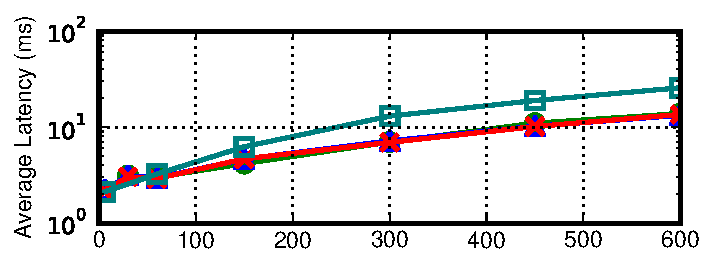
\includegraphics[width=0.90\columnwidth]{figs/lan-threads-lats.pdf}\vspace{-1em}
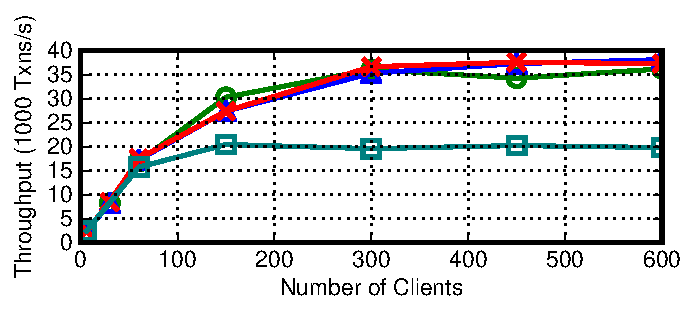
\includegraphics[width=0.90\columnwidth]{figs/lan-threads-thru.pdf}
\begin{center}\textbf{Between \texttt{us-east} and \texttt{us-west-2}}\end{center}\vspace{-1.5em}
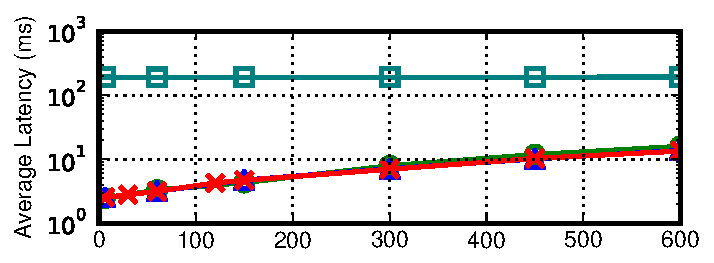
\includegraphics[width=0.90\columnwidth]{figs/wan-threads-lats.pdf}\vspace{-1em}
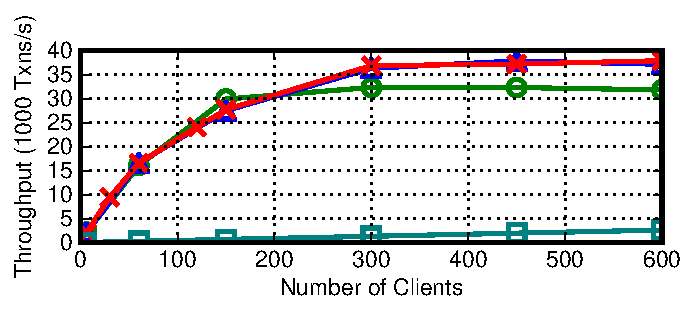
\includegraphics[width=0.90\columnwidth]{figs/wan-threads-thru.pdf}
\caption{YCSB performance for two clusters of three servers each
  deployed within a single datacenter and cross-datacenters.}
\label{fig:wan-exp}
\end{figure}

As Figure~\ref{fig:wan-exp} shows, within a single datacenter, a
mastered implementation achieves approximately double the latency and
slightly over half of the throughput of a HAT implementation. This is
because, given two replicas for each key, the mastered implementation
serves requests from only one. The mastered implementation still
achieves $19,797$ transactions per second---over 6,000 per
master---and is only $15.56$ms slower at peak compared to eventual
consistency. However, eventual consistency and HAT models achieve
substantially higher throughput--$37,575$ and $36,178$ transactions
per second, respectively--and lower latency---$48.3\%$ and $47.2\%$
respectively. This difference is unsurprising because, in these weaker
models, all servers can serve both reads and writes, effectively
doubling the capacity of the system. The weaker models still propagate
new values between replicas, but this process is asynchronous and,
aside from consuming disk I/O and network bandwidth, does not
substantially impact clients. As expected, HAT models perform
similarly to eventual consistency: our Read Committed implementation
buffers client writes and adds no additional server-side overhead,
while TA requires additional metadata with each write but has less
than 5\% performance impact compared to eventual consistency.

In comparison, over multiple datacenters, the cost of coordination
increases. The HAT and eventual consistency implementations continue
to enjoy local RTTs only, and, with the exception of a slight
performance degradation in TA---which we believe is attributable to
Java garbage collection overheads in TA's inbound anti-entropy
buffers---performance remains unchanged. However, each YCSB update to
a remote replica ($\frac{2}{3}$ in one datacenter, $\frac{1}{3}$ in
the other) of requiring a remote RTT between Virginia and Oregon (or
vice-versa) to reach the master. This leads to a latency increase of
around $166$ms ($746\%$) per transaction compared to a
single-datacenter deployment. In order to attain reasonable throughput
for the mastered deployment, we had to greatly increase the number of
concurrent clients accessing the database, and we found that threading
and socket overheads quickly overwhelmed the database server. Over a
wide-area network, the increased cost of RTTs dramatically affects
system efficiency.

This brief set of experiments is not meant as an exhaustive study, but
it validates our earlier intuition regarding the cost of violating
HAT-compliance. As Deutsch points out, ignoring factors such as
latency can ``cause big trouble and painful learning
experiences''~\cite{fallacies-deutsch}---in a single-site context,
paying the cost of coordination may be tenable, but, especially as
services are geo-replicated, the costs increase. 



\section{Related Work}
\label{sec:relatedwork}

We have discussed traditional mechanisms for distributed
coordination and several related systems in
Section~\ref{sec:eval-existing}, but, in this section, we further discuss
related work. In particular, we discuss related work on highly
available semantics, mechanisms for concurrency control, and
techniques for scalable distributed operations.

Weak consistency and high availability have been well
studied. Serializability has long been known to be
unachievable~\cite{davidson-survey} and Brewer's CAP Theorem has
attracted considerable attention~\cite{gilbert-cap}. Recent work on
PACELC expands CAP by considering connections between ``weak
consistency'' and low latency~\cite{abadi-pacelc}, while several
studies examine weak isolation guarantees~\cite{adya,
  ansicritique}. There are a wide range of coordination-avoiding
``optimistic replication'' strategies~\cite{optimistic} and several
recent efforts at further understanding these strategies in light of
current practice and the proliferation of ``eventually consistent''
stores~\cite{bailis-ec, bernstein-survey}. Notably, Bernstein and
Das~\cite{bernstein-survey} specifically highlight the importance of
stickiness~\cite{sessionguarantees, vogels-defs}---which we formalize
in Section~\ref{sec:sticky}.  Aside from our earlier workshop paper
discussing transactional availability, real-world ACID, and HAT RC and
I-CI~\cite{hat-hotos}---which this work expands with additional
semantics, algorithms, and analysis---we believe this paper is the
first to explore the connections between transactional semantics, data
consistency, and (Gilbert and Lynch~\cite{gilbert-cap}) availability.

%, linearizability, consistent snapshots, and recency
%bounds~\cite{ceri-mechanism, chen-mechanism}.

There has been a recent resurgence of interest in distributed
multi-object semantics, both in academia~\cite{kraska-s3, gstore,
  eiger, walter,calvin, swift} and industry~\cite{orleans,spanner}. As
discussed in Section~\ref{sec:modernacid}, classic ACID databases
provide strong semantics but their lock-based and traditional
multi-versioned implementations are unavailable in the presence of
partitions~\cite{bernstein-book, gray-isolation}. Notably, Google's
Spanner provides strong one-copy serializable transactions. While
Spanner is highly specialized for Google's read-heavy workload, it
relies on two-phase commit and two-phase locking for read/write
transactions~\cite{spanner}. As we have discussed, the penalties
associated with this design are fundamental to serializability. For
users willing to tolerate unavailability and increased latency,
Spanner, or similar ``strongly consistent''
systems~\cite{kemme-classification}---including Calvin~\cite{calvin},
G-Store~\cite{gstore}, HBase, HStore~\cite{hstore},
Orleans~\cite{orleans}, Postgres-R~\cite{kemme-thesis},
Walter~\cite{walter}, and a range of snapshot isolation
techniques~\cite{daudjee-session}---reasonable
choices.

With HATs, we seek an alternative set of transactional semantics that
are still useful but do not violate requirements for high availability
or low latency. Recent systems proposals such as Swift~\cite{swift},
Eiger~\cite{eiger}, and Bolt-on Causal Consistency~\cite{bolton}
provide transactional causal consistency guarantees with varying
availability and represent a new class of sticky HAT systems. There
are infinitely many HAT models (i.e., always reading value 1 is
incomparable with always returning value 2), but a recent report from
UT Austin shows that no model stronger than causal consistency is
achievable in a sticky highly available, \textit{one-way convergent}
system~\cite{cac}. This result is promising and complementary to our
results for general-purpose convergent data stores. Finally, Burkhardt
et al. have concurrently developed an axiomatic specification for
eventual consistency; their work-in-progress report contains alternate
formalism for several HAT guarantees~\cite{burkhardt-txns}.


% Ceri discuss distributed database update mechanisms with respect to
% linearizability, consistent snapshots (i.e., cut isolation), and
% recency bounds~\cite{ceri-mechanism}.  Chen and Pu also classify
% distributed replica maintenance from perspectives of
% linearizability,% recency guarantees, and replica
% divergence~\cite{chen-mechanism}.



%, with increasing interest in returning to transactional
%designs~\cite{spanner, walter, foundation-article, krikellas-bargain,
%  eiger}




\section{Future Work}
\label{sec:futurework}

There are several promising avenues for future work in HATs:

\textbf{What are the limits of achievable HAT models, and how are they
  defined?}  In this work, we have taxonomized several well-defined
and well-documented semantic properties. This is useful as it
contextualizes decades of existing database and distributed systems
design and algorithms but does not provide guidance as to what
consistency models are the ``strongest''---or admit the smallest set
of executions---within each availability class. A recent report from
UT Austin shows that no model stronger than causal consistency can be
achieved in a sticky highly available, one-way convergent
system~\cite{cac}, but there are infinite highly available and sticky
highly available models to consider. For example, always returning the
value $1$ in response to reads is incomparable with (i.e., neither
stronger nor weaker than) causal consistency: returning $1$ does not
respect causality, and causal consistency returns values other than
$1$. Always returning the value $2$ is similarly incomparable, and, as
an example, we can enumerate models that return all integers and real
numbers--an uncountably infinite set of models. Given these infinite
models, are there meaningful properties that delineate the boundaries
between classes of highly available systems? Is there a
``meta-property'' that exactly characterizes what properties are
achievable with high availability or sticky high availability? This is
an area of ongoing research within the Berkeley HAT project.

\textbf{What are the costs and benefits within HAT designs?} There are
many possible combinations of HAT guarantees, and the performance and
ease of implementation of a HAT system will vary depending on which
guarantees it provides. For example, as we have discussed, the cost in
moving from a sticky high available implementation of highly available
guarantees to a truly highly available system seems expensive for some
models (e.g., metadata requirements or visibility requirements may
become problematic). Further experimentation regarding the set of
useful and achievable HAT guarantees will shed further light on this
question.

\textbf{Where do semantics-based concurrency control and weakened
  failure models lie in the HAT landscape?} The vast
literature on semantics-based concurrency control provides hints as to
when coordination can be avoided while providing ``strongly
consistent'' outcomes for limited failure scenarios. We have performed
a narrow case study in this work, but a general taxonomization of
techniques such as escrow transactions~\cite{escrow},
Sagas~\cite{sagas}, and other long-running transaction support could
help answer the challenge of programming in a weakly consistent
environment. HAT guarantees can also be strengthened by considering
weaker failure models such as bounded asynchrony or models in which
the underlying hardware provides explicit service-level
agreements. Additionally, while we have focused on systems that
provide a single availability mode, there are several interesting
hybrids to consider. For example, a system may provide ``best-effort''
stickiness (or serializability) in the absence of partitions, but, in
the presence of partitions, ``lose'' guarantees by having clients
reconnect to an available replica. This strategy provides stronger
guarantees in the absence of partitions but, to provide availability,
sacrifices them in the event of partitions.



\section{Conclusions and Future Work}
\label{sec:conclusion}

The current state of database software offers uncomfortable and
unnecessary choices between availability and transactional semantics.
Through our analysis and experiments, we have demonstrated how goals
of high availability will remain a critical aspect of many future data
storage systems. We expose a broad design space of Highly Available
Transactions (HATs), which can offer the key benefits of highly
available distributed systems---``always on'' operation during
partitions and low-latency operations (often orders of magnitude lower
than non-compliant)---while also providing a family of transactional
isolation levels and replica semantics that have been adopted in
practice.  We also identify many semantic guarantees that are
unachievable with high availability, including Lost Update and Write
Skew anomaly prevention, concurrent update prevention, and bounds on
data recency. Despite these limitations, and somewhat surprisingly,
many of the default (and sometimes strongest) semantics provided by
today's traditional database systems are achievable as HATs, hinting
that distributed databases need not compromise availability, low
latency, or scalability in order to serve many existing applications.

In this paper, we have largely focused on previously defined isolation
and data consistency models from the consistency from the database and
distributed systems communities. Their previous definitions and, in
many cases, widespread adoption hints at their utility to
end-users. However, we believe there is considerable work to be done
to improve the programmability of highly available systems. Isolation
and data consistency are means by which \textit{application-level}
consistency is achieved but are typically not end goals for end-user
applications. Our results hint that a mix of HAT and non-HAT semantics
(the latter used sparingly) is required for practical applications,
but the decision to employ each and the system architectures for a
hybrid approach remain open problems. While we have studied the
analytical and experiment behavior of several HAT models, there is
substantial work in further understanding the performance and design
of systems within the large set of HAT models. Weakened failure
assumptions as in escrow or in the form of bounded network asynchrony
could enable richer HAT semantics at the cost of general-purpose
availability. Alternatively, there is a range of possible solutions
providing strong semantics during partition-free periods and weakened
semantics during partitions. Based on our understanding of what is
desired in the field and newfound knowledge of what is possible to
achieve, we believe HATs represent a large and useful design space for
exploration.

%% In this paper we expose a broad design space of Highly Available Transactional 
%% Systems (HATs), which can offer the key benefits of
%% highly available distributed systems---partition tolerance and low-latency 
%% writes---while also providing a family of transactional isolation 
%% levels and replica semantics that have been widely used in practice. 
%% In taxonomizing this design space, we show that many transactional 
%% guarantees are achievable with high availability, while a few, 
%% like preventing Lost Update and Write Skew, are not. 

%% There has been some debate in the database community regarding the importance
%% of availability in modern databases; there is also concern about the utility of
%% relaxed isolation.  Our analysis and experiments in Sections~\ref{sec:motivation} 
%% and~\ref{sec:evaluation} convince us that the availability goals of the NoSQL
%% movement will remain a critical aspect of many important systems going forward, and 
%% that the isolation levels available via HATs can have significant practical impact
%% in delivering useful transactional semantics to application developers.

%% Much of the prior research in distributed transactions has focused on prototyping 
%% individual points in the design space, with a focus on providing serializability
%% at the expense of availability.  Our goal in this paper has been to take a broader view. 
%% We taxonomize the joint design space of replica consistency and transactional isolation,
%% and identify what is possible and impossible to achieve semantically via HATs.  From
%% a research perspective, this offers a long-overdue connection between storage 
%% semantics studied in the database and distributed systems communities.
%% With this understanding in hand, the next challenge is to return to issues of 
%% performance and systems architecture within the HATs design space.  Based on our 
%% understanding of what is desired in the field and what is possible to achieve, we 
%% believe this is an area of great opportunity in the coming years.



foo~\cite{adya}

% The following two commands are all you need in the
% initial runs of your .tex file to
% produce the bibliography for the citations in your paper.
\bibliographystyle{abbrv}
% vldb_sample.bib is the name of the Bibliography in this case
\bibliography{hat-vldb}  
% You must have a proper ".bib" file
%  and remember to run:
% latex bibtex latex latex
% to resolve all references

\subsection{References}

Generated by bibtex from your ~.bib file. Run latex, then bibtex, then
latex twice (to resolve references).

%APPENDIX is optional.
% ****************** APPENDIX **************************************
% Example of an appendix; typically would start on a new page
%pagebreak

\begin{appendix}

\end{appendix}

\end{document}
